\documentclass[a4paper]{article}

\usepackage[english]{babel}
\usepackage[utf8]{inputenc}
\usepackage{amsmath}
\usepackage{graphicx}
\usepackage[colorinlistoftodos]{todonotes}
\usepackage{hyperref}
\usepackage{float}
\usepackage[margin=1in]{geometry}
\hypersetup{urlcolor=blue, linkcolor=blue, colorlinks=true} % Colors hyperlinks in blue -
\title{Open Source Workshop}

\author{Pablo Hernandez, Elsa Guillot}

\date{\today}

\begin{document}
\maketitle

%\begin{abstract}

%\end{abstract}

\section{Introduction}

Welcome to the magic world of open source software. We will guide you through mainstream open-source software and the Linux OS.
\subsection{What is open source?}

Free and open-source software (FOSS) is computer software that can be classified as both free software and open source software. That is, anyone is freely licensed to use, copy, study, and change the software in any way, and the source code is openly shared so that people are encouraged to voluntarily improve the design of the software.This is in contrast to proprietary software, where the software is under restrictive copyright and the source code is usually hidden from the users.

The benefits of using FOSS can include decreasing software costs, increasing security and stability (especially in regard to malware), protecting privacy, and giving users more control over their own hardware. Free, open-source operating systems such as Linux are used utilized today, powering millions of servers, desktops, smartphones (e.g. Android), and other devices. Free software licences and open-source licenses are used by many software packages.

\subsection{Why should I use open-source software?}
Good question! Mumbling...\\
I think the answer is plainly, because it is more reliable. Not ethics involved. You do not depend on the private company bussiness model...
\begin{itemize}
\item Adaptability.
\item Long term.
\item No commercial dead-ends, always available.
\item Reproducible and reviewed, better code.
\end{itemize}Î
And of course, you are contributing to the open knowledge, with all the good repercussion that it has in the global scale.
\subsection{Two kind of open licenses: Copyleft vs Permissive}

\textbf{Copyleft:} an arrangement whereby software or artistic work may be used, modified, and distributed freely on condition that anything derived from it inherits the same license.\\
\textbf{Permissive:} no restrictions, the free software can be re-licensed and copyrighted by anyone.\\

Copyleft licenses, such as GPL, are well considered by the community. Projects with these kind of licenses have usually more chances to attract collaboration from individuals, knowing that their work won't be 'exploited' by third-parties in the future. Copyleft licenses has sometimes called as viral, because any software that makes use of GPL licensed code has to become GPL as well.\\

In the permissive side we have BSD, Apache, MIT, EPL, and a myriad of other licenses. Code under this license can find support from private companies that would take advantage of the development, re-licensing it under their copyright license and monetize from it. Of course, the original code is also free for the competence, which is good for the consumer at the end.\\

There are heated debates in the open source community about what of these two flavors are 'more' free.\\
If you are thinking about freeing your work to take advantage of the collaborative support of the open source community, or just because you want to contribute to the open knowledge, you should weight the pros and cons of both licenses and choose the one that benefits the most to your project.\\
Around 70\% of the FOSS projects are under permissive licenses.

\section{Linux Installation}
\subsection{Origins}
Linux was initially developed by Linus Torvalds in 1991 while attending Helsinki University. Unix, an OS developed by AT\&T (Bell labs) in 1969 was getting spread in academia, but it was prohibitively expensive for the independent user. The first Linux kernel was developed inside Minix, a Unix clone that was free for educational purposes only.\\
Linux adopted the GNU GPLv2 (copyleft) license. The OS was free to use, free to distribute and free to commercialize, with the only condition that the modifications inherits the same copyleft condition.\\
The kernel community (the core of linux) is, by far, the biggest open source community in the world. Linus himself is not coding anymore, he has become a manager and supervisor of the new developments. To handle that, he created git, a version control software that allows big collaborations, we will introduce git later on.

There are many other Unix-like OS. Mac OS for example was born as a fork from a BSD (permissive license) Unix Clone, that is why both OS share some similarities. Windows Microsoft is not Unix-like.

\subsection{Linux distributions -- Distros}
Ubuntu, RedHat, Mint, are all names of different distros that you may have heard. A distribution is a central set of software, built on top of the linux kernel, that adds functionality and provides a friendly interface for the user. 
Distros usually target users with different requirements. The three main points of divergence between them are three:
\begin{itemize}
    \item Software and kernel updates.\\ A web developer may need cutting-edge updates of the software he/she is using. However, a company developing a heavy piece of new software depending on an external library, don't want to face the new bugs of the last release of that library.
    \item Package Manager and software repositories.\\ A package manager is a collection of software tools that automates the process of installing, upgrading, configuring and removing software packages, taking care of mismatches and inter-dependencies. In Linux you usually don't download installers from the web, you use the package manager instead. The packages are bundled into repositories, you have official repositories from your chosen distro, but also you can access to bundles made and maintained for other users. YUM in RedHat derivates (Fedora, Centos), APT for Debian forks (Ubuntu, Mint) are the most famous package managers. Ubuntu package repositories are BIG (Mint has access to them from the version we are installing), so you will be well fed. 
    \item Desktop Environment.\\ Windows Microsoft name is inspired by its desktop environment. In Linux there are many more options. The most influent have been Gnome and KDE, with Unity, and Cinnamon getting more adepts, these are very complete environments. In the light side, faster but with less graphical interfaces for some things, we have Xcfe and LXDE. You can even try the non-floating windows desktops, such as i3 or monads. The best thing about the open source branching, is that you can find whatever suits you the best.
\end{itemize}

Linux is not only for computer programmers anymore, thanks to the effort of the distros, it is easy to install, thanks to the kernel development, hardware recognition is not a hassle anymore, and thanks to the desktop environment, the navigation through the applications is mint. Since it is \textbf{free}, more and more universities and institutions are using it in a daily basis. There exists non-free distributions of Linux, such as RedHat and Suse, to handle incompatibilities of copyrighted libraries with GNU, and also with extra features to automatize management in big computer networks.\\
\subsubsection{Mint}
For this workshop we have chosen Mint -Ubuntu flavor-. It has a standard update policy, with software upgrading every 6 months. There is also a Debian based flavor, that has a rolling updates policy, where the software is continually updated. The package manager is APT, same as ubuntu, and able to access to the huge Ubuntu official repositories. The desktop environment will be Cinnamon, a modern gnome shell fork, that provides a user friendly -windows like- experience.

But of course, there are more alternatives, other distributions are available for you to test if you want; we have bootable DVDS of Centos, Fedora and Kubuntu. But there are plenty of other distros, with new ones arising every month.
\subsection{Virtual Machine}
A virtual machine is basically a software that emulates an Operating System. It creates a completely functional and independent 'virtual' machine inside your current OS, as if you had a new computer (Linux) within your computer (Windows or Mac). You start the virtual machine as you would execute any other software. That means Linux will become available to you at a double click distance from your current setup. \\
The advantages of using a virtual machine are:
\begin{itemize}
\item You do not need to handle sensible parts of your computer.
\item Your data is safer, because you don't have to deal with hard-drive partitions required to install a new OS.
\item You can try things out with Linux without risking of breaking your system, as the Linux part will be independent of your primary OS
\item You can have several OS to play with, try new Linux distros, or even setup Linux from scratch with the ArchLinux distro with no risk (if you are able to do this without re-starting the process a couple of times.. MANA).
\end{itemize}

The virtual machine will get information from the host OS, such as network credentials and hardware related controllers. Great software have been developed now, to make it as hassle-free as possible.\\

\subsubsection{Virtual Box}
We will use VM Virtual Box, a really good, free, open-source, tool from Oracle that works with any OS. Alternative Virtual Machines: Parallels (\$) for Mac, VMWare (free and multi-platform).

We have written a complete VirtualBox setup guide, available at: \url{https://github.com/phcerdan/open-source-workshop/blob/master/vbox-linux-installation-guide/main.pdf}. Download from it!

\section{Open source tools}
\subsection{Zotero}
\url{https://www.zotero.org/}

Zotero is a library manager to handle those tons of pdf papers that you accumulate over time. It works flawlessly integrated with the open source browser Firefox. It is able to store into your library the paper you are reading into your browser with just one click.\\

Zotero has two versions, firefox integrated and standalone version. The standalone version have plugins for firefox,chrome,and safari. I use the firefox integrated version, and I would show and recommend this one, but there should be no much difference between both.\\

\textbf{Firefox Integrated:}\\
I highly recommend to create a firefox account (Preferences > Sync), to synchronize the following steps for all your computers (A virtual machine counting as a new computer!)
Using Firefox, go to zotero page and click in the option Add to Firefox in the left, and that's it!\\
You can add useful add-ons, using the Firefox>Tools>Add-ons (Ctrl-Shift-A by default), and search for zotero. Zotfile is a must!

Useful shortcuts:\\
\begin{figure}[H]
    \centering
    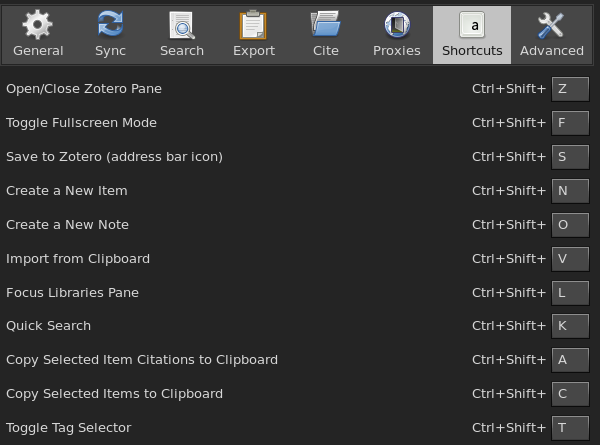
\includegraphics[width=0.5\linewidth]{zotero_shortcuts.png}
    \caption{Zotero default shortcuts}
    \label{fig:zotero_shortcuts}
\end{figure}

\subsubsection{Integration with text processors}
\label{ssub:integration_with_text_processors}
It is straight forward! Go to zotero preferences > Cite. And install the integration you want. A plugin will appear in the text processor, where you can insert cites, and also the complete bibliography.
\begin{figure}[H]
    \centering
    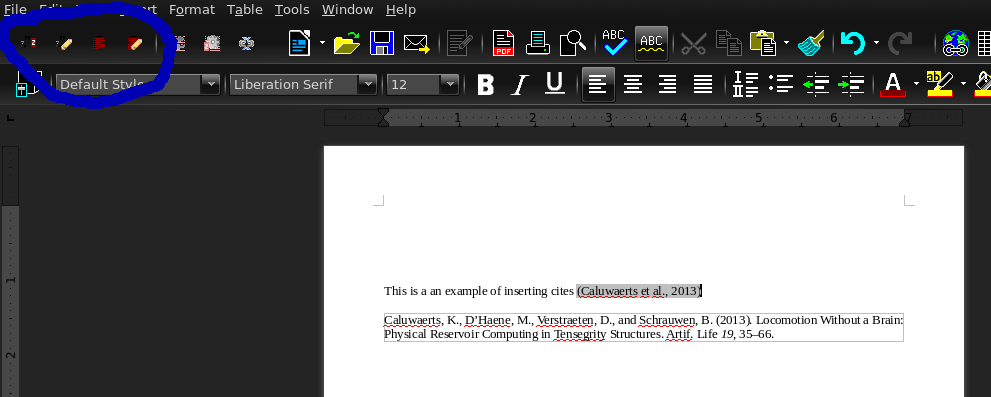
\includegraphics[width=0.6\linewidth]{zotero_word.png}
    \caption{A plugin will be installed in your word processor, and it will sync with your Zotero library}
    \label{fig:zotero_word}
\end{figure}
\subsubsection{For big libraries: storage options}
\label{ssub:for_big_libraries_storage_options}

If you have a massive pdf collection, you can be interested in buying some extra space. But there are still free options. Storage pricing for big libraries in Zotero:\\
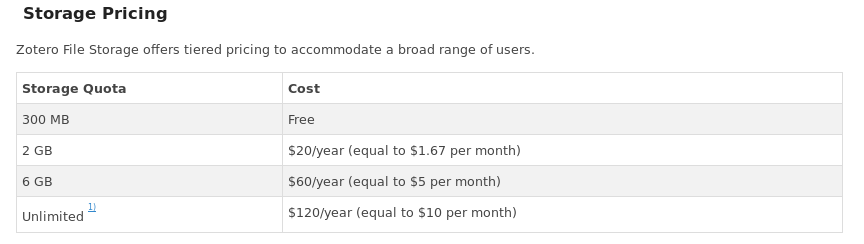
\includegraphics[width=0.9\textwidth]{zotero_price.png} \\

Other webDAV services: CloudMe:\\
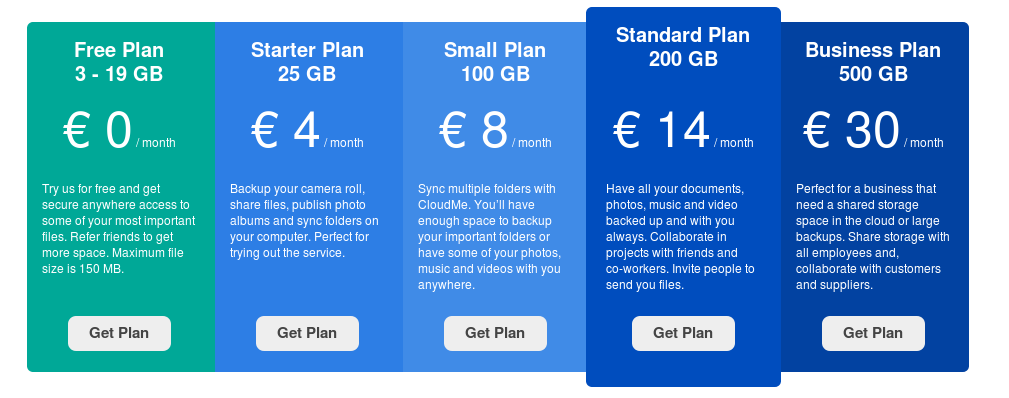
\includegraphics[width=0.9\textwidth]{zotero_price_cloudme.png}\\

Using Dropbox and Zotfile:\\
If you already have dropbox extra space and not willing to pay extra storage room in a webDAV (reccomended), you can use Dropbox as the storage folder and use Zotfile to rename the pdfs to something legible. This option is the one that I will show, and even though it is a bit brittle, you don't need zotero to access your pdfs.

\subsection{GitHub}
Git is a version control system to work with highly non-linear and parallel inputs.It was created by Linus Torvalds to manage the thousand of people that contributed to the Linux Kernel \url{http://git-scm.com/}. Git allows the different developers work simultaneously in the same code, and then merge their work together. You can create forks, and branches from a version, develop a special feature on it, and put it back later without interfering with others jobs meanwhile.\\

Github is a web server where the software controlled by git can be stored \url{https://github.com/}. It has become the place where the open source community collaborate and communicate, as an alternative to sourceforge.net.\\
It promotes free and open source project by offering free services to open source project only. There are also free services for students (free hosting of 5 projects plus a set of tools for programming).\\
Version systems is the only way to collaborate in code, but it can be used for one person project, to keep track of all the changes you have made to a document, or if coding to test crazy ideas creating branches from your stable version.\\

\section{Program}
\begin{itemize}
\item 3-4pm Linux Party.\\
Discover Linux. Fire up the installations
\item 4-5pm Open Source.\\
Explnation of what's open source, and presentation of GitHub and Zotero
\item 5-6pm Trouble shoooting the installs.\\
Give it a try to an other distribution (live CD). Find out if people want more stuff happening, if so what do they want? Blabla with your neighbours.
\item 6-late BQQ at Pablo's
\end{itemize}

\end{document}
